% These lines tell TeXShop to typeset with xelatex, and to open and 
% save the source with Unicode encoding.

%!TEX TS-program = xelatex
%!TEX encoding = UTF-8 Unicode
%! program = pdflatex

%% Get all the page and style setup from a common file
\documentclass[10pt,a4paper,oneside]{memoir}

% Use fontspec for loading Trebuchet MS
\usepackage{fontspec,xltxtra,xunicode}
\defaultfontfeatures{Mapping=tex-text}
\setromanfont[Mapping=tex-text]{Trebuchet MS}
\setsansfont[Scale=MatchLowercase,Mapping=tex-text]{Trebuchet MS}
\setmonofont[Scale=MatchLowercase]{Courier New}

\usepackage{unicode-math}
\usepackage{mathtools}
\setmathfont{xits-math.otf}

% Use xcolor package for color definitions
\usepackage[cmyk]{xcolor}
\definecolor{myblack}{RGB/cmyk}{0,0,0/0,0,0,1}
\definecolor{mycyan}{RGB/cmyk}{0.89,0.96,1.0/0.09,0,0,0} % #e4f5fd
\definecolor{myorange}{RGB/cmyk}{0.77,0.47,0.09/0.20,0.57,1,0.05} % #c57917


% Use graphicx for importing images
\usepackage{graphicx}

% Use hyperref for links
\usepackage{hyperref}
\hypersetup{colorlinks=true,
            linkcolor=myblack,
            urlcolor=myblack}

% Use tabularx for tables and colortbl for adding color

\usepackage{tabulary}
\usepackage{colortbl}
% Set the rule properties for tables
\setlength\arrayrulewidth{0.4mm}
\setlength{\heavyrulewidth}{0.4mm}
\setlength{\lightrulewidth}{0.2mm}
\arrayrulecolor{myorange}
% Make a new rule similar to misrule but with heavy weight
\newcommand{\otoprule}{\midrule[\heavyrulewidth]}

% Use listings for pretty-printing of code 
\usepackage{listings}

% Add some extra commands for changing the row styles of tables
% This is from http://www.tug.org/pracjourn/2007-1/mori/mori.pdf
\newcolumntype{+}{>{\global\let\currentrowstyle\relax}}
\newcolumntype{^}{>{\currentrowstyle}}
   \newcommand{\rowstyle}[1]{\gdef\currentrowstyle{#1}%
   #1\ignorespaces
   }

% Usage in table adds '+' and '^' for delimiters, like this:
% \begin{tabular}{+l^c^c^c}
% \toprule\rowstyle{\bfseries}%
% Quantity & Symbol & Unit & Value \\\otoprule%
% ...
% \end{tabular}

% Defines the length used for hanging the tex block from the chapter / section headings
\newlength{\textblockhang}
\newlength{\textblockheight}
\newlength{\textblockwidth}
\setlength{\textblockhang}{10mm}
\setlength{\textblockheight}{224mm}
\setlength{\textblockwidth}{150mm}

\setlength{\droptitle}{5cm}

% Define the page layout
\settrimmedsize{297mm}{210mm}{*}

\newlength{\textblockleftmargin}
\setlength{\textblockleftmargin}{\paperwidth}
\addtolength{\textblockleftmargin}{\textblockhang}
\addtolength{\textblockleftmargin}{-\textblockwidth}
\setlength{\textblockleftmargin}{0.5\textblockleftmargin}

\setlength{\trimtop}{0pt}
\setlength{\trimedge}{\stockwidth}
\addtolength{\trimedge}{-\paperwidth}
\settypeblocksize{\textblockheight}{\textblockwidth}{*}
\setulmargins{4cm}{*}{*}
\setlrmargins{\textblockleftmargin}{*}{*}
\setmarginnotes{17pt}{51pt}{\onelineskip}
\setheadfoot{\onelineskip}{2\onelineskip}
\setheaderspaces{*}{2\onelineskip}{*}
\checkandfixthelayout

% Define the style for footer and header
% Default footer has the company address
\newcommand{\footcontents}
{SoLoud Audio Engine - http://soloud-audio.com}

% Length \headfootwidth is used for the width of the footer
\newlength{\headfootwidth}
\setlength{\headfootwidth}{\textwidth}
\addtolength{\headfootwidth}{\textblockhang}

\makepagestyle{mypage}
\makefootrule{mypage}{\headfootwidth}{0.4mm}{1.5mm}
\makeevenfoot{mypage}{
  \color{black}\thepage
}{
  \color{black}\small \footcontents
}{  
}
\makeoddfoot{mypage}{
}{
  \color{black}\small \footcontents
}{
  \color{black}\thepage
}
\makeevenhead{mypage}{}{}{}
\makeoddhead{mypage}{}{}{}
\makeheadfootruleprefix{mypage}{\color{myblack}}{\color{myblack}}
\makerunningwidth{mypage}{\headfootwidth}
\makeheadposition{mypage}{flushright}{flushright}{flushright}{flushright}

\aliaspagestyle{part}{mypage}
\aliaspagestyle{chapter}{mypage}
\pagestyle{mypage}

% Define title page hooks
\pretitle{\begin{center}\begin{Spacing}{-0.5}\huge}
\posttitle{\par\vspace{-3mm}\color{myorange}\rule{\textwidth}{0.4mm}\color{black}\end{Spacing}\end{center}}
\preauthor{\begin{center}\begin{Spacing}{-1}\Large}
\postauthor{\par\end{Spacing}\end{center}}
\predate{\begin{center}\begin{Spacing}{-1}\large}
\postdate{\par\end{Spacing}\end{center}
  \begin{figure}[b]
    \begin{center}
    
\includegraphics[width=12.0cm]{SoLoudLogo.pdf}
    \end{center}
  \end{figure}
}

% Set section numbering up to and including subsection
\setsecnumdepth{subsection}
\maxtocdepth{subsection}
\settocdepth{subsection}

% Create a custom chapter style. This is based on hangnum from memoir.
\makechapterstyle{mychapter}{%
  \renewcommand*{\chaptitlefont}{\normalfont\LARGE\bfseries}
  \renewcommand*{\chapnumfont}{\chaptitlefont}
  % allow for 99 chapters!
  \settowidth{\chapindent}{\chapnumfont 999}
  \renewcommand*{\printchaptername}{}
  \renewcommand*{\chapternamenum}{}
  \renewcommand*{\chapnumfont}{\chaptitlefont}
  \renewcommand*{\printchapternum}{%
    \noindent\llap{\makebox[\chapindent][l]{%
    \chapnumfont \thechapter}}}
  \renewcommand*{\afterchapternum}{}
  \renewcommand{\insertchapterspace}{}
  \setlength{\afterchapskip}{10pt}
  \setlength{\beforechapskip}{10pt}
}

% Tweak the indents by \textblockhang outside the margin.
\chapterstyle{mychapter}
\setlength{\chapindent}{\textblockhang}
\setsecindent{-\textblockhang}
\setsubsecindent{-\textblockhang}
\setsubsubsecindent{-\textblockhang}

\setlength{\parindent}{0mm}
\setlength{\parskip}{10pt}
\definecolor{codebg}{rgb}{0.9,0.9,0.9}
\lstset{
	basicstyle=\small, 
	stringstyle=\ttfamily, 
	backgroundcolor=\color{codebg}, 
	commentstyle=\color{blue},
	language=C++,
	framexleftmargin=6pt,
	framextopmargin=2pt,
	framexbottommargin=2pt,
	frame=tb,
	framerule=0pt
	}


\usepackage{longtable}

\usepackage{float}
\restylefloat{table} 
\restylefloat{figure}

%% Set the image paths
\graphicspath{{images/}}

% \input{GrammarCheckSetup}
    
%%% DOCUMENT TITLE
\title{SoLoud Audio Engine}
\author{Jari Komppa}
%\date{November 19, 2018}
%\date{August 2012} % Delete this line to display the current date

\usepackage{titletoc}
\titlecontents{chapter}[3em]{\addvspace{10pt}\bfseries}
    {\contentslabel{2.5em}}{\hspace{-2.5em}}{\hfill\contentspage}
\dottedcontents{section}[6.3em]{}{3.3em}{0.7pc}
\dottedcontents{subsection}[10.5em]{}{4.2em}{0.7pc}
\renewcommand\chapternumberline[1]{\numberline{#1}}

\usepackage[ ]{titlesec}  %
\titleformat{\chapter}[display]
  { \normalsize \huge  \color{black}}
  {\flushright \normalsize \color{black} \MakeUppercase { \chaptertitlename } \hspace{1 ex} { \fontsize{60}{60}\selectfont \color{black} \sffamily  \thechapter }} {10 pt}{\huge}

\usepackage{blowup}
\blowUp{target=a5}

%%% BEGIN DOCUMENT
\begin{document}
\lstset{
    language=C++,
    basicstyle=\small,
    keywordstyle=\color{black},
    identifierstyle=\color{black},
    commentstyle=\color{myorange},
    stringstyle=\ttfamily,
    showstringspaces=false,
    tabsize=2,
    backgroundcolor=\color{mycyan}}

\frontmatter
\begin{titlingpage}
\maketitle
\pagestyle{plain}
\newpage

These pages were intentionally left blank.

\newpage

(Except for this text)

\newpage

� 2018 Komppa, Jari\\
%Kustantaja: BoD - Books on Demand, Helsinki, Suomi\\
%Valmistaja: BoD - Books on Demand, Norderstedt, Saksa\\
%ISBN: 978-952-80-0359-5
\end{titlingpage}


% Use * to avoid the entries themselves to get inserted in TOC
\tableofcontents*
% \listoffigures*
% \listoftables*

%===============================================================================
% All parts of the document are included as separate files.
\mainmatter

% !TEX root = SoLoud.tex
%===============================================================================

\chapter{Introduction}

SoLoud is an easy to use, free, portable c/c++ audio engine for games.

\section {How easy?}
The engine has been designed to make simple things easy, while not making harder things impossible. Here's a code snippet that initializes the library, loads a sample and plays it:

\begin{lstlisting}{frame=single, framerule=1pt}
// Declare some variables
SoLoud::Soloud soloud; // Engine core
SoLoud::Wav sample;    // One sample

// Initialize SoLoud (with SDL)
SoLoud::sdl_init(&soloud);

sample.load("pew_pew.wav"); // Load a wave file
soloud.play(sample);        // Play it
\end{lstlisting}

The primary form of use the interface is designed for is "fire and forget" audio. In many games, most of the time you don't need to modify a sound's parameters on the fly - you just find an event, like an explosion, and trigger a sound effect. SoLoud handles the rest.

If you need to alter some aspect of the sound after the fact, the "play" function returns a handle you can use. For example:

\begin{lstlisting}{frame=single, framerule=0pt}
int handle = soloud.play(sample);         // Play the sound
soloud.setVolume(handle, 0.5f);           // Set volume; 1.0f is "normal"
soloud.setPan(handle, -0.2f);             // Set pan; -1 is left, 1 is right
soloud.setRelativePlaySpeed(handle, 0.9f);// Play a bit slower; 1.0f is normal
\end{lstlisting}

If the sound doesn't exist anymore (either it's ended or you've played so many sounds at once it's channel has been taken over by some other sound), the handle is still safe to use - it just doesn't do anything.

\section{How free?}
SoLoud is released under the ZLib/LibPNG license. That means you can use it in free or commercial applications as much as you want. You can modify it. You don't need to give the changes back. You don't need to release the source code. You don't need to add a splash screen. You don't need to mention it in your printed manual.

Basically the only things the license forbids are suing me, or claiming that you made SoLoud. If you redistribute the source code, the license needs to be there. But not with the binaries.

Parts of the SoLoud package were not made by me, and those either have a similar license, or more permissive (such as Unlicense, CC0, WTFPL or Public Domain).

\section{There's a Catch, Right?}

SoLoud quite probably doesn't have all the features you'd find in a commercial library like FMOD or WWISE. There's no artist tools or engine integration. There's no 3d audio. Output is, currently, limited to stereo.

It quite probably isn't as fast. As of this writing, it has no specialized assembler optimizations, for any platform.

It certainly doesn't come with the support you get from a commercial library.

If you're planning to make a multi-million budgeted console game, this library is (probably) not for you. Feel free to try it though =)

% !TEX root = SoLoud.tex
%===============================================================================

\chapter{Quick Start}

Note: SoLoud supports several different "back ends", but this quickstart guide assumes you're using SDL; the primary difference is that to use a different back-end, you call the desired back-end's init function (instead of SDL's).

\section{Download SoLoud}

First, you need to download SoLoud sources. You can find the downloads on the http://soloud-audio.com/download.html page.

\section{Add files to your project}

You can go the lazy way and just add all of the sources to your project, or you can copy the things you need to a single directory and include those. You'll need the core files, and quite likely the wav files. If you need the speech synth, include those, too.

\section{Include files}

In order to use a certain feature of SoLoud, you need to include its include file. You might have, for instance:

\begin{lstlisting}{frame=single, framerule=1pt}
#include "soloud.h"
#include "soloud_wav.h"
\end{lstlisting}

\section{Variables}

You need at least the SoLoud engine core, and one or more of the sound source variables. If you're using five different sound effect wav files, you need five SoLoud::Wav objects. You can play one object any number of times, even on top of each other.

Where to place these is up to you. Globals work, as do allocation from heap, including in a class as members, etc.

\begin{lstlisting}{frame=single, framerule=1pt}
SoLoud::Soloud gSoloud;
SoLoud::Wav gWave;
\end{lstlisting}

\section{Initialize SoLoud}

After your SDL\_Init call, include a call to initialize SoLoud. The call takes a pointer to the SoLoud core object.

\begin{lstlisting}{frame=single, framerule=1pt}
SoLoud::sdl_init(&gSoloud);
\end{lstlisting}

\section{Set up sound sources}

This step varies from one sound source to another, but basically you'll load your wave files here.

\begin{lstlisting}{frame=single, framerule=1pt}
gWave.load("pew_pew.wav");
\end{lstlisting}

\section{Play sounds}

Now you're ready to play the sounds. Place playing commands wherever you need sound to be played.

\begin{lstlisting}{frame=single, framerule=1pt}
gSoloud.play(gWave);
\end{lstlisting}

Note that you can play the same sound several times, and it doesn't cut itself off.

\section{Take control of the sound}

You can adjust various things about the sound you're playing if you take the handle.

\begin{lstlisting}{frame=single, framerule=1pt}
int x = gSoloud.play(gWave);
gSoloud.setPan(x, -0.2f);
\end{lstlisting}

Read the soloud.h header file (or this documentation) for further things you can do.

\section{Cleanup}

After you've done, remember to clean up. If you don't, the audio thread may do stupid things while the application is shutting down.

\begin{lstlisting}{frame=single, framerule=1pt}
gSoloud.deinit();
\end{lstlisting}

\section{Enjoy}

And you're done!
% !TEX root = SoLoud.tex
%===============================================================================

\chapter{Frequently Asked Questions}

\section{What does it play?}

Currently, SoLoud includes support for uncompressed 8 and 16 bit RIFF Wav files, as well as Ogg Vorbis files. Both of these only support a limited feature set of said formats, so you may experience some issues with strange files.

Additionally, SoLoud comes with a speech synthesizer.

The interface for audio sources is relatively simple, so new formats and noise generators, as well as audio filters, can be made.

An example sin/saw/triangle/square generator is also available, as part of the "piano" example.

Since there are several liberally-licensed audio sources available, the number of formats SoLoud will support is likely to grow in the future.

\section{What dependencies does it have?}

There's no external library dependencies (apart from stdlib). However, to get audio out of your speakers, a back-end is needed. Back-ends that currently exist include SDL, windows multimedia and portaudio, and SoLoud has been designed so that making new back-ends would be as painless as possible.

\section{Is there a DLL / C-Interface?}

Not yet. This has been requested though, so one may appear at some point.

\section{What's the animal in the logo?}

A fennec fox. Google it. They're cute!

\section{Is there a mailing list?}

There's a google group, at http://groups.google.com/d/forum/soloud

Main development occurs on GitHub, at https://github.com/jarikomppa/soloud and the issue tracker is in use.

Finally, there's \#soloud on ircnet, if you want to pop by.

\section{Are these real questions?}

Surprisingly, yes.
\include{temp/dirstruct}
\include{temp/premake}
% !TEX root = SoLoud.tex
%===============================================================================

\chapter{Legal}

SoLoud, like everything else, stands on the shoulders of giants; however, care has been taken to only incorporate source code that is under liberal licenses, namely ZLib/LibPNG, CC0 or public domain, or similar, like WTFPL or Unlicense, where you don't need to include mention of the code in your documentation or splash screens or any such nonsense.

\section{SoLoud Proper}

SoLoud proper is licensed under the ZLib/LibPNG license. The code is a clean-room implementation with no outside sources used.

\scriptsize
\begin{verbatim}
SoLoud audio engine
Copyright (c) 2013 Jari Komppa

This software is provided 'as-is', without any express or implied
warranty. In no event will the authors be held liable for any damages
arising from the use of this software.

Permission is granted to anyone to use this software for any purpose,
including commercial applications, and to alter it and redistribute it
freely, subject to the following restrictions:

   1. The origin of this software must not be misrepresented; you must not
   claim that you wrote the original software. If you use this software
   in a product, an acknowledgment in the product documentation would be
   appreciated but is not required.

   2. Altered source versions must be plainly marked as such, and must 
   not be misrepresented as being the original software.

   3. This notice may not be removed or altered from any source
   distribution.
\end{verbatim}
\normalsize

\section{OGG Support}
The OGG support in the Wav and WavStream sound sources is based on stb\_vorbis by Sean Barrett, and it's in the public domain. You can find more information (and latest version) at http://nothings.org/stb\_vorbis/

\section{Speech Synthesizer}
The speech synth is based on rsynth by the late Nick Ing-Simmons (et al). He described the legal status as:

\scriptsize
\begin{verbatim}
    This is a text to speech system produced by
    integrating various pieces of code and tables
    of data, which are all (I believe) in the
    public domain.
\end{verbatim}
\normalsize

Since then, the rsynth source code has passed legal checks by several open source organizations, so it "should" be pretty safe.

The primary copyright claims seem to have to do with text-to-speech dictionary use, which I've removed completely.

I've done some serious refactoring, clean-up and feature removal on the source, as all I need is "a" free, simple speech synth, not a "good" speech synth. Since I've removed a bunch of stuff, this is probably safer public domain release than the original.

I'm placing my changes in public domain as well, or if that's not acceptable for you, then CC0: http://creativecommons.org/publicdomain/zero/1.0/.

The SoLoud interface files (soloud\_speech.*) are under the same ZLib/LibPNG license as the other SoLoud bits.

\section{Fast Fourier Transform (FFT)}

FFT calculation is provided by a fairly simpple implementation by Stephan M. Bernsee, under the Wide Open License:

\scriptsize
\begin{verbatim}
COPYRIGHT 1996 Stephan M. Bernsee <smb [AT] dspdimension [DOT] com>

						The Wide Open License (WOL)

Permission to use, copy, modify, distribute and sell this software and its
documentation for any purpose is hereby granted without fee, provided that
the above copyright notice and this license appear in all source copies. 
THIS SOFTWARE IS PROVIDED "AS IS" WITHOUT EXPRESS OR IMPLIED WARRANTY OF
ANY KIND. See http://www.dspguru.com/wol.htm for more information.
\end{verbatim}
\normalsize


% !TEX root = SoLoud.tex
%===============================================================================

\chapter{Concepts}

\section{Back end}

SoLoud itself "only" performs audio mixing and some resource handling. For it to be useful, it needs one or more sound source and a back end. Some other systems call back-ends 'sink's. Examples of back-ends would be winmm, portaudio, wasapi and SDL audio. SoLoud comes with several back-ends, and is designed to make back-ends relatively easy to implement.

\section{Channel}

One audio stream can contain one or more channels. Typical audio sources are either mono (containing one channel) or stereo (containing two channels), but surround sound audio sources may practically have any number of channels.

\section{Stream}

SoLoud can play audio from several sound sources at once (or, in fact, several times from the same sound source at the same time). Each of these sound instances is a "stream". The number of concurrent streams is limited, as having unlimited streams would cause performance issues, as well as lead to unnecessary clipping.

The default number of concurrent streams - maximum number of "voices" - is 64, but this can be adjusted via a defined constant in the soloud.h file. The hard maximum number is 4096, but if more are required, SoLoud can be modified to support more. But seriously, if you need more than 4096 sounds at once, you're probably going to make some serious changes in any case.

If all channels are already playing and the application requests another sound to play, SoLoud finds the oldest sound and kills it. Since this may be your background music, you can protect channels from being killed by using the soloud.setProtect call.

\section{Clipping}

Audio hardware always has a limited dynamic range. If you think of a signed 16-bit variable, for instance, you can only store values from -32k to +32k in it; if you try to put values outside this range in, things tend to break. Same goes for audio.

\begin{figure}[H]
  \begin{center}
  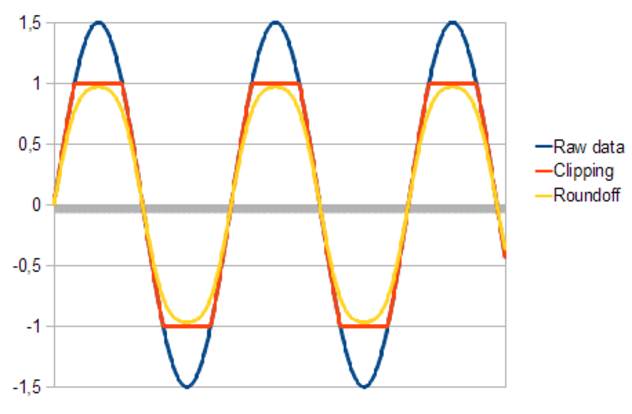
\includegraphics[width=12.0cm]{clipping.pdf}
  \end{center}
\end{figure}
  
SoLoud handles all audio as floats, but performs clipping before passing the samples out, so all values are in the -1..1 range. There's two ways SoLoud can perform the clipping; the most straghtforward is simply to set all values outside this range to the border value, or alternatively a roundoff calculation can be performed, which "compresses" the loud sounds. The more quiet sounds are largely unchanged, while the loud end gets less precision. The roundoff clipper is used by default.

The roundoff clipper does, however, alter the signal and thus "damages" the sound. A more proper way of doing things would be to use the basic clipper and adjust the global volume to avoid clipping. The roundoff clipper, however, is easier to use.

\section{Sample}

The real world has continious signals, whuch would require infinite amount of storage to store (unless you can figure out some kind of complicated mathematical formula that represents the signal). So, we store discrete samples of signals instead. These samples have traditionally been 8, 16 or 24 bit, but high-end audio is tending towards floating point samples.

SoLoud also uses floating point samples internally. First and foremost, it makes everything much simpler, and second, modern computing devices have become fast enough that this is not really an issue anymore.

Floating point samples also take more space than, for instance, 16 bit samples, but memory and storage sizes have also grown enough to make this a feasible approach. Nothing stops the audio sources from keeping data in a more "compressed" format and performing on-the-fly conversion to float, if memory requirements are a concern.

\section{Sample Rate}

The sample rate represents the number of samples used, per second. Typical sample rates are 8000hz, 22050hz, 44100hz and 48000hz. Higher the sample rates mean clearer sound, but also bigger files, more memory and higher processing power requirements.

\section{Play Speed}

In addition to a base sample rate, which represents the "normal" playing speed, SoLoud includes a "relative play speed" option. This simply changes the sample rate. However, if you replace your sounds with something that has a different "base" sample rate, using the relative play speed will retain the effect of playing the sound slower (and lower) or faster (and higher).

\section{Relative Play Speed}

SoLoud lets you change the relative play speed of samples. Please note that asking for a higher relative play speed is more expensive than a lower one.

\section{Resampling}

SoLoud has to perform resampling when mixing. In an ideal case, all of the sources and the destination sample rate are the same, and no resampling is needed, but this is often not true. Currently, SoLoud supports "point sample" resampling, which means it simply skips or repeats samples as needed, as well as "linear interpolation", which calculates linear interpolation of samples. Higher quality resamplers are planned.

\section{Pan}

Where the sound is coming from in the stereo sound, ranging from left speaker only to right speaker only. SoLoud uses an algorithm to calculate the left/right channel volume so that the overall volume is retained across the field. You can also set the left/right volumes directly, if needed.

\section{Handle}

SoLoud uses throwaway handles to control sounds. The handle is an integer, and internally tracks the channel and sound id, as well as an "uniqueness" value.

If you try to use a handle after the sound it represents has stopped, the operation is quietly discarded (or if you're requesting information, some kind of generic value is returned). You can also query the validity of a handle.

\section{Sound Source and Instance}

SoLoud uses two kinds of classes for the sounds. Sound sources contain all the information related to the sound in question, such as wave sample data, while sound instances contain information about an "instance" of the sound.

As an analogue, if you think of an old vinyl record, the sound source is the record, and you can put as many playheads - the instances - on the record. All of the playheads can also move at different speeds, output to a different pan position and volume.

\section{Latency}

Audio latency generally means the time it takes from triggering a sound to the sound actually coming out of the speakers. The smaller the latency, the better.

Unfortunately, there's always some latency. The primary source of latency (that a programmer can have any control over) is the size of audio buffer. Generally speaking, the smaller the buffer, the lower the latency, but at the same time, the smaller the buffer, the more likely the system hits buffer underruns (ie, the play head marches on but there's no data ready to be played) and the sound breaks down horribly.

Assuming there's no other sources of latency (and there quite likely is), with 2048 sample buffer and 44100Hz playback, the latency is around 46 milliseconds, which is tolerable in most cases. A 100ms latency is already easily noticeable.

\section{Filter}

Audio streams can also be modified on the fly for various effects. Typical uses are different environmental effects such as echoes or reverb, or low pass (bassy sound) / high pass (tinny sound) filters, but basically any kind of modification can be done; the primary limitation is the processor power.

SoLoud lets you hook several filters to a single audio stream, as well as to the global audio output.

\section{Mixing Bus}

In addition to mixing audio streams together at the "global" level, SoLoud includes mixing busses which let you mix together groups of audio streams. These serve several purposes.

The most typical use would be to let the user change the volume of different kinds of audio sources - music, sound effects, speech. In this case, you would have one mixing bus for each of these audio source groups, and simply change the volume on the mixing bus, instead of hunting down every sound separately.

When using environmental effects filters, you most likely won't want the background music to get filtered; the easiest way to handle this is to apply the filters to the mixing bus that plays the sound effects. This will also save on processing power, as you don't need to apply the environmental audio filters on every sound effect separately.

It's also possible that you have some very complex audio sources, such as racing cars. In this case it makes sense to place all the audio streams that play from one car into a mixing bus, and then adjust the panning (or, eventually, 3d position) of the mixing bus.
\include{temp/concepts3d}
\include{temp/voicemanagement}

\include{temp/examples}

\include{temp/foreign_interface}
\include{temp/bmx_api}
\include{temp/c_api}
\include{temp/cs_api}
\include{temp/d_api}
\include{temp/gamemaker_api}
\include{temp/python_api}
\include{temp/ruby_api}
\include{temp/rpgmaker_api}
\include{temp/codegen}

% !TEX root = SoLoud.tex
%===============================================================================

\chapter{Core: Basics}

\section{SoLoud::Soloud Object}

In order to use SoLoud, you have to create a SoLoud::Soloud object. The object must be cleaned up or destroyed before your back-end is shut down; the safest way to do this is to call soloud.deinit() manually before terminating.

The object may be global, member variable, or even a local variable, it can be allocated from the heap or the stack, as long as the above demand is met. If the back-end gets destroyed before the back-end clean-up call is made, the result is undefined. As in, bad. Most likely, a crash. Bluescreens in Windows are not out of the question.

\begin{lstlisting}{frame=single, framerule=1pt}
SoLoud::Soloud *soloud = new SoLoud::Soloud; // object created
SoLoud::sdl_init(soloud);   // back-end initialization
...
soloud->deinit();           // clean-up
delete soloud;              // this cleans up too
\end{lstlisting}

Seriously: remember to call the cleanup function. The SoLoud object destructor also calls the cleanup function, but if you perform your application's teardown in an unpredictable order (such as having the SoLoud object be a global variable), the back-end may end up trying to use resources that are no longer available. So, it's best to call the cleanup function manually.

\section{Soloud.play()}

The play function can be used to start playing a sound source. The function has more than one parameter, with typical default values set to most of them.

\begin{lstlisting}{frame=single, framerule=1pt}
int play(AudioSource &aSound, 
         float aVolume = 1.0f, // Full volume 
         float aPan = 0.0f,    // Centered
         int aPaused = 0,      // Not paused
         int aBus = 0);        // Primary bus
\end{lstlisting}

The play function returns a channel handle which can be used to adjust the parameters of the sound while it's playing. The most common parameters can be set with the play function parameters, but for more complex processing you may want to start the sound paused, adjust the parameters, and then un-pause it.

\begin{lstlisting}{frame=single, framerule=1pt}
int h = soloud.play(sound, 1, 0, 1);  // start paused
soloud.setRelativePlaySpeed(h, 0.8f); // change a parameter
soloud.setPause(h, 0);                // unpause
\end{lstlisting}

\section{Soloud.seek()}

You can seek to a specific time in the sound with the seek function. Note that the seek operation may be rather heavy, and some audio sources will not support seeking backwards at all.

\begin{lstlisting}{frame=single, framerule=1pt}
int h = soloud.play(sound, 1, 0, 1); // start paused
soloud.seek(h, 3.8f);                // seek to 3.8 seconds
soloud.setPause(h, 0);               // unpause
\end{lstlisting}

\section{Soloud.stop()}

The stop function can be used to stop a sound.

\begin{lstlisting}{frame=single, framerule=1pt}
soloud.stop(h); // Silence!
\end{lstlisting}

\section{Soloud.stopAll()}

The stop function can be used to stop all sounds. Note that this will also stop the protected sounds.

\begin{lstlisting}{frame=single, framerule=1pt}
soloud.stopAll(); // Total silence!
\end{lstlisting}

\section{Soloud.stopSound()}

The stop function can be used to stop all sounds that were started through a certain sound source. Will also stop protected sounds.

\begin{lstlisting}{frame=single, framerule=1pt}
soloud.stopSound(duck); // silence all the ducks
\end{lstlisting}

\section{Soloud.setGlobalVolume() / Soloud.getGlobalVolume()}

These functions can be used to get and set the global volume. The volume is applied before clipping. Lowering the global volume is one way to combat clipping artifacts.

\begin{lstlisting}{frame=single, framerule=1pt}
float v = soloud.getGlobalVolume(); // get the current global volume
soloud.setGlobalVolume(v * 0.5f);   // halve it
\end{lstlisting}

Note that the volume is not limited to 0..1 range. Negative values may result in strange behavior, while huge values will likely cause distortion.

\section{Soloud.setPostClipScaler() / Soloud.getPostClipScaler()}

These functions can be used to get and set the post-clip scaler. The scaler is applied after clipping. Sometimes lowering the post-clip result sound volume may be beneficial. For instance, recording video with some video capture software results in distorted sound if the volume is too high.

\begin{lstlisting}{frame=single, framerule=1pt}
float v = soloud.getPostClipScaler(); // get the current post-clip scaler
soloud.setPostClipScaler(v * 0.5f);   // halve it
\end{lstlisting}

Note that the scale is not limited to 0..1 range. Negative values may result in strange behavior, while huge values will likely cause distortion.
% !TEX root = SoLoud.tex
%===============================================================================

\chapter{Core: Attributes}

\section{Soloud.getVolume() / Soloud.setVolume()}

These functions can be used to get and set a sound's current volume setting.

\begin{lstlisting}{frame=single, framerule=1pt}
float v = soloud.getVolume(h); // Get current volume
soloud.setVolume(h, v * 2);    // Double it
\end{lstlisting}

Note that the volume is the "volume setting", and the actual volume will depend on the sound source. Namely, a whisper will most likely be more quiet than a scream, even if both are played at the same volume setting.

If an invalid handle is given to getVolume, it will return 0.

\section{Soloud.getPan() / Soloud.setPan()}

These functions can be used to get and set a sound's current pan setting.

\begin{lstlisting}{frame=single, framerule=1pt}
float v = soloud.getPan(h); // Get current pan
soloud.setPan(h, v - 0.1);  // Little bit to the left
\end{lstlisting}

The range of the pan values is -1 to 1, where -1 is left, 0 is middle and and 1 is right. Setting value outside this range may cause undefined behavior.

SoLoud calculates the left/right volumes from the pan to keep a constant volume; to set the volumes directly, use setPanAbsolute.

If an invalid handle is given to getPan, it will return 0.

\section{Soloud.setPanAbsolute()}

These function can be used to set the left/right volumes directly.

\begin{lstlisting}{frame=single, framerule=1pt}
soloud.setPanAbsolute(h, 1, 1); // full blast
\end{lstlisting}

Note that this does not affect the value returned by getPan.

If an invalid handle is given to getPan, it will return 0.

\section{Soloud.getSamplerate() / Soloud.setSamplerate()}

These functions can be used to get and set a sound's base sample rate.

\begin{lstlisting}{frame=single, framerule=1pt}
float v = soloud.getSamplerate(h); // Get the base sample rate
soloud.setSamplerate(h, v * 2);    // Double it
\end{lstlisting}

Setting the value to 0 will cause undefined behavior, likely a crash.

To adjust the play speed, while leaving the base sample rate alone, 
use setRelativePlaySpeed instead.

If an invalid handle is given to getSamplerate, it will return 0.

\section{Soloud.getRelativePlaySpeed() / Soloud.setRelativePlaySpeed()}

These functions can be used to get and set a sound's relative play speed.

\begin{lstlisting}{frame=single, framerule=1pt}
float v = soloud.getRelativePlaySpeed(h); // Get relative play speed
soloud.setRelativePlaySpeed(h, v * 0.5f); // Halve it
\end{lstlisting}

Setting the value to 0 will cause undefined behavior, likely a crash.

Change the relative play speed of a sample. This changes the effective sample rate while leaving the base sample rate alone.

Note that playing a sound at a higher sample rate will require SoLoud to request more samples from the sound source, which will require more memory and more processing power. Playing at a slower sample rate is cheaper.

If an invalid handle is given to getRelativePlaySpeed, it will return 1.

\section{Soloud.getProtectChannel() / Soloud.setProtectChannel()}

These functions can be used to get and set a sound's protection state.

\begin{lstlisting}{frame=single, framerule=1pt}
int v = soloud.getProtectChannel(h);   // Get the protection state
if (v) soloud.setProtectChannel(h, 0); // Disable if protected
\end{lstlisting}

Normally, if you try to play more sounds than there are channels, SoLoud will kill off the oldest playing sound to make room. This will most likely be your background music. This can be worked around by protecting the sound.

If all sounds are protected, the result will be undefined.

If an invalid handle is given to getProtectChannel, it will return 0.

\section{Soloud.getPause() / Soloud.setPause()}

The setPause function can be used to pause, or unpause, a sound.

\begin{lstlisting}{frame=single, framerule=1pt}
if (soloud.getPause(h)) hum_silently();
soloud.setPause(h, 0); // resumes playback
\end{lstlisting}

Note that even if a sound is paused, its channel may be taken over. Trying to resume a sound that's no longer in a channel doesn't do anything.

If the handle is invalid, the getPause will return 0.

\section{Soloud.setPauseAll()}

The setPauseAll function can be used to pause, or unpause, all sounds.

\begin{lstlisting}{frame=single, framerule=1pt}
soloud.setPauseAll(h, 0); // resumes playback of all channels
\end{lstlisting}

Note that this function will overwrite the pause state of all channels at once. If your game uses this to pause/unpause the sound while the game is paused, do note that it will also pause/unpause any sounds that you may have paused/unpaused separately.

\section{Soloud.setFilterParameter()}

Sets a parameter for a live instance of a filter. The filter must support changing of live parameters; otherwise this call does nothing.

\begin{lstlisting}{frame=single, framerule=1pt}
soloud.setFilterParameter(bar,lp,cutoff,1000); 
// set bar's low pass to cut at 1000hz
\end{lstlisting}

\section{Soloud.getFilterParameter()}
Gets a parameter from a live instance of a filter. The filter must support changing of live parameters; otherwise this call returns zero.
\begin{lstlisting}{frame=single, framerule=1pt}
float v = soloud.getFilterParameter(bar,lp,cutoff); 
// get bar's low pass cutoff
\end{lstlisting}


% !TEX root = SoLoud.tex
%===============================================================================

\chapter{Core: Faders}

\section{Overview}

Faders are a convenient way of performing some common audio tasks without having to add complex code into your application.

The most common use for the faders is to fade audio in or out, adding nice touches and polish.

Let's say you're exiting a bar and entering the street.

\begin{lstlisting}{frame=single, framerule=1pt}
soloud.fadeVolume(bar_ambience, 0, 2); // fade bar out in 2 seconds
soloud.scheduleStop(bar_ambience, 2);  // stop the bar ambience after fadeout
street_ambience = soloud.play(cars, 0);// start steet ambience at 0 volume
soloud.setProtectChannel(street_ambience, 1); // protect it
soloud.fadeVolume(street_ambience, 1, 1.5f); // fade street in in 1.5
\end{lstlisting}

Or let's say you're quiting your game.

\begin{lstlisting}{frame=single, framerule=1pt}
soloud.fadeGlobalVolume(0, 1); // Fade out global volume in 1 second
\end{lstlisting}

The faders are only evaluated once per mix function call - in other words, whenever the back end requests samples from SoLoud, which is likely to be in chunks of 20-100ms, which is smoothly enough for most uses.

The exception is volume (which includes panning), which gets interpolated on per-sample basis to avoid artifacts.

The starting value for most faders is the current value.

\section{Soloud.fadeVolume()}

Smoothly change a channel's volume over specified time.

\begin{lstlisting}{frame=single, framerule=1pt}
soloud.fadeVolume(orchestra, 1, 60); // The orchestra creeps in for a minute
\end{lstlisting}

The fader is disabled if you change the channel's volume with setVolume()

\section{Soloud.fadePan()}

Smoothly change a channel's pan setting over specified time.

\begin{lstlisting}{frame=single, framerule=1pt}
soloud.setPan(racecar, -1); // set start value
soloud.fadePan(racecar, 1, 0.5); // Swoosh!
\end{lstlisting}

The fader is disabled if you change the channel's panning with setPan() or setPanAbsolute()

\section{Soloud.fadeRelativePlaySpeed()}

Smoothly change a channel's relative play speed over specified time.

\begin{lstlisting}{frame=single, framerule=1pt}
soloud.fadeRelativePlaySpeed(hal, 0.1, 6); // Hal's message slows down
\end{lstlisting}

The fader is disabled if you change the channel's play speed with setRelativePlaySpeed()

\section{Soloud.fadeGlobalVolume()}

Smoothly change the global volume over specified time.

\begin{lstlisting}{frame=single, framerule=1pt}
soloud.fadeGlobalVolume(0, 2); // Fade everything out in 2 seconds
\end{lstlisting}

The fader is disabled if you change the global volume with setGlobalVolume()

\section{Soloud.schedulePause()}

After specified time, pause the channel

\begin{lstlisting}{frame=single, framerule=1pt}
soloud.fadeVolume(jukebox, 0, 2); // Fade out the music in 2 seconds
soloud.schedulePause(jukebox, 2);    // Pause the music after 2 seconds
\end{lstlisting}

The scheduler is disabled if you set the pause state with setPause() or setPauseAll().

\section{Soloud.scheduleStop()}

After specified time, stop the channel

\begin{lstlisting}{frame=single, framerule=1pt}
soloud.fadeVolume(applause, 0, 10); // Fade out the cheers for 10 seconds
soloud.scheduleStop(applause, 10);     // Stop the sound after 10 seconds
\end{lstlisting}

There's no way (currently) to disable this scheduler.

\section{Soloud.oscillateVolume()}

Set fader to oscillate the volume at specified frequency.

\begin{lstlisting}{frame=single, framerule=1pt}
soloud.oscillateVolume(murmur, 0, 0.2, 5); // murmur comes and goes
\end{lstlisting}
The fader is disabled if you change the channel's volume with setVolume()

\section{Soloud.oscillatePan()}

Set fader to oscillate the panning at specified frequency.

\begin{lstlisting}{frame=single, framerule=1pt}
soloud.oscillatePan(ambulance, -1, 1, 10); // Round and round it goes
\end{lstlisting}
The fader is disabled if you change the channel's panning with setPan() or setPanAbsolute()

\section{Soloud.oscillateRelativePlaySpeed()}
Set fader to oscillate the relative play speed at specified frequency.

\begin{lstlisting}{frame=single, framerule=1pt}
soloud.oscillateRelativePlaySpeed(vinyl, 0.9, 1.1, 3); // Wobbly record
\end{lstlisting}

The fader is disabled if you change the channel's play speed with setRelativePlaySpeed()

\section{Soloud.oscillateGlobalVolume()}
Set fader to oscillate the global volume at specified frequency.

\begin{lstlisting}{frame=single, framerule=1pt}
soloud.oscillateGlobalVolume(0.5, 1.0, 0.2); // Go crazy
\end{lstlisting}

The fader is disabled if you change the global volume with setGlobalVolume()

\include{temp/voicegroups}
% !TEX root = SoLoud.tex
%===============================================================================

\chapter{Core: Misc}

\section{Soloud.getStreamTime()}

The getStreamTime function can be used to get the current play position, in seconds.

\begin{lstlisting}{frame=single, framerule=1pt}
float t = soloud.getStreamTime(h); // get time
if (t == hammertime) hammer();
\end{lstlisting}

Note that due to being a floating point value, playing a long stream may cause precision problems, and eventually cause the "time" to stop. This will happen in about 6 days. The precision problems will start somewhat earlier.

Also note that the granularity is likely to be rather high (possibly around 45ms), so using this as the sole clock source for animation will lead to rather low framerate (possibly around 20hz). To fix this, either use some other clock source and only sync with the stream time occasionally, or use some kind of low-pass filter.

\section{Soloud.isValidChannelHandle()}

The isValidChannelHandle function can be used to check if a handle is still valid.

\begin{lstlisting}{frame=single, framerule=1pt}
if (soloud.isValidChannelHandle(h)) delete foobar;
\end{lstlisting}

If the handle is invalid, the getPause will return 0.

\section{Soloud.getActiveVoiceCount()}

Returns the number of concurrent sounds that are playing at the moment.

\begin{lstlisting}{frame=single, framerule=1pt}
if (soloud.getActiveVoiceCount() == 0) enjoy_the_silence();
\end{lstlisting}

If the handle is invalid, the getPause will return 0.

\section{Soloud.setGlobalFilter()}

Sets, or clears, the global filter.

\begin{lstlisting}{frame=single, framerule=1pt}
soloud.setGlobalFilter(0, &echochamber); // set first filter
\end{lstlisting}

Setting the global filter to NULL will clear the global filter. The default maximum number of global filters active is 4, but this can be changed in a global constant in soloud.h.

\section{Soloud.calcFFT()}

Calculates FFT of the currently playing sound (post-clipping) and returns a pointer to the result.

\begin{lstlisting}{frame=single, framerule=1pt}
float * fft = soloud.calcFFT();
int i;
for (i = 0; i < 256; i++)
  drawline(0, i, fft[i] * 32, i);
\end{lstlisting}

The FFT data has 256 floats, from low to high frequencies.

SoLoud performs a mono mix of the audio, passes it to FFT, and then calculates the magnitude of the complex numbers for application to use. For more advanced FFT use, SoLoud code changes are needed.

The returned pointer points at a buffer that's always around, but the data is only updated when calcFFT() is called.

For the FFT to work, you also need to initialize SoLoud with the Soloud::ENABLE\_VISUALIZATION flag. Otherwise the source data for the FFT calculation will not be gathered.

\section{Soloud.getWave()}

Gets 256 samples of the currently playing sound (post-clipping) and returns a pointer to the result.

\begin{lstlisting}{frame=single, framerule=1pt}
float * wav = soloud.getWave();
int i;
for (i = 0; i < 256; i++)
  drawline(0, i, wav[i] * 32, i);
\end{lstlisting}

The returned pointer points at a buffer that's always around, but the data is only updated when getWave() is called. The data is the same that is used to generate visualization FFT data.

For this function to work properly, you also need to initialize SoLoud with the \linebreak Soloud::ENABLE\_VISUALIZATION flag. Otherwise the source data will not be gathered, and the result is undefined (probably zero).

\include{temp/core3d}

% !TEX root = SoLoud.tex
%===============================================================================

\chapter{SoLoud::AudioSource}

All audio sources share some common functions. Some of the functionality depends on the audio source itself; it may be that some parameter does not make sense for a certain audio source, or it may be that it has not been implemented for other reasons.

For example, if you stream a live radio station, looping does not make much sense.

\section{AudioSource.setLooping()}

This function can be used to set a sample to play on repeat, instead of just playing once.

\begin{lstlisting}{frame=single, framerule=1pt}
amenbreak.setLooping(1); // let the beat play on
\end{lstlisting}

Note that some audio sources may not implement this behavior.

\section{AudioSource.setFilter()}

This function can be used to set or clear the filters that should be applied to the sounds generated via this audio source.

\begin{lstlisting}{frame=single, framerule=1pt}
speech.setFilter(0, blackmailer); // Disguise the speech
\end{lstlisting}

Setting the filter to NULL will clear the filter. This will not affect already playing sounds.
By default, up to four filters can be applied. This value can be changed through a constant in the soloud.h file.

\section{AudioSource.setSingleInstance()}

This function can be used to tell SoLoud that only one instance of this sound may be played at the same time.

\begin{lstlisting}{frame=single, framerule=1pt}
menuselect.setSingleInstance(1); // Only play it once, sam
\end{lstlisting}

% !TEX root = SoLoud.tex
%===============================================================================

\chapter{Creating New Audio Sources}

SoLoud is relatively easy to extend by creating new sound sources. Each sound source consists of two parts: an audio source class, and an audio instance class.

Studying the existing audio sources' source code, in addition to this chapter, will be helpful in creating new ones.

\section{AudioSource}

\begin{lstlisting}{frame=single, framerule=1pt}
class Example : public AudioSource
{
public:
  virtual AudioInstance *createInstance();
};
\end{lstlisting}

The only mandatory member of an audio source is the createInstance function.

The audio source class is meant to contain all and any data that represents the sound in general and can be reused by the instances; for instance, with wave files, the wave data is stored with the audio source, while audio instances just read the data.

Note that there's no setLooping() function - that's inherited from AudioSource, and sets the SHOULD\_LOOP flag.

The audio source is also responsible for setting the mChannels and mBaseSamplerate values. These values get copied to all of the instances of this audio source.

\section{AudioSource.createInstance()}

The createInstance function typically creates and returns its counterpart, the audio instance. Usually it also gives a pointer to itself to the audio instance.

\section{AudioSourceInstance}

\begin{lstlisting}{frame=single, framerule=1pt}
class ExampleInstance : public AudioSourceInstance
{
public:
  virtual void getAudio(float *aBuffer, int aSamples);
  virtual int hasEnded();
  virtual void seek(float aSeconds, float *mScratch, int mScratchSize);
  virtual int rewind();
};
\end{lstlisting}

The getAudio and hasEnded methods are mandatory. Seek and rewind are optional.

The audio instance is meant as the "play head" for a sound source. Most of the data should be in the audio source, while audio instance may contain more logic.

\section{AudioSourceInstance.getAudio()}

SoLoud requests samples from the sound instance using the getAudio function. If the instance generates more than one channel (i.e, stereo sound), the expected sample data first has the first channel samples, then second channel samples, etc. 

So, if 1024 samples are requested from a stereo audio source, the first 1024 floats should be for the first channel, and the next 1024 samples should be for the second channel.

The getAudio function is also responsible for handling looping, if the audio source supports it. See the implementations of existing sound sources for more details.

If the audio source runs out of data, the rest of the buffer should be set to zero.

\section{AudioSourceInstance.hasEnded()}

After mixing, SoLoud asks all audio instances whether they have ended, and if they have, it will free the object and free the channel. Supporting looping will likely affect the implementation of this function.

\section{AudioSourceInstance.seek()}

Optionally, you can implement a seek function. The base implementation will simply request (and discard) samples from the sound source until the desired position has been reached; for many sound sources, a smarter way exists.

\section{AudioSourceInstance.rewind()}

To enable the base implementation of seek to seek backwards from the current play position, sound source may implement the rewind function. In most cases the rewind is easier to implement than actual smart seeking.

% !TEX root = SoLoud.tex
%===============================================================================

\chapter{SoLoud::Wav}

The SoLoud::Wav class represents a wave sound effect. The source files may be in 8 or 16 bit raw RIFF WAV files, or compressed Ogg Vorbis files.

The sounds are loaded and converted to float samples, which means that every second of a 44100hz stereo sound takes about 350kB of memory. The good side is, after loading, these samples are very lightweight, as their processing is mostly just a memory copy.

For lenghty samples like background music, you may want to use SoLoud::WavStream instead.

\section{Wav.load()}

The wav loader takes just one parameter, the file name:

\begin{lstlisting}{frame=single, framerule=1pt}
void load(const char *aFilename); // File to load
\end{lstlisting}

If loading fails, the sample will be silent.

\begin{lstlisting}{frame=single, framerule=1pt}
SoLoud::Wav boom;
boom.load("boom.wav");
\end{lstlisting}

If the loading function is called while there are instances playing, the result is undefined (most likely a crash).

\section{Wav.loadMem()}

Alternate way of loading samples is to read from a memory buffer.

\begin{lstlisting}{frame=single, framerule=1pt}
void loadMem(unsigned char *aMem, int aLength); // Sample to load
\end{lstlisting}

If loading fails, the sample will be silent.

\begin{lstlisting}{frame=single, framerule=1pt}
SoLoud::Wav boom;
boom.loadMem(boomMemoryResource, boomMemoryResourceLength);
\end{lstlisting}

If the loading function is called while there are instances playing, the result is undefined (most likely a crash).

% !TEX root = SoLoud.tex
%===============================================================================

\chapter{SoLoud::WavStream}

The SoLoud::WavStream class represents a wave sound effect that is streamed off disk while it's playing. The source files may be in 8 or 16 bit raw RIFF WAV files, or compressed Ogg Vorbis files.

The sounds are loaded in pieces while they are playing, which takes more processing power than playing samples from memory, but they require much less memory.

For short or often used samples, you may want to use SoLoud::Wav instead.

\section{WavStream.load()}

The wav loader takes just one parameter, the file name:

\begin{lstlisting}{frame=single, framerule=1pt}
void load(const char *aFilename); // File to load
\end{lstlisting}

If loading fails, the sample will be silent.

\begin{lstlisting}{frame=single, framerule=1pt}
SoLoud::WavStream muzak;
muzak.load("elevator.ogg");
\end{lstlisting}

If the loading function is called while there are instances playing, the result is undefined (most likely a crash).

% !TEX root = SoLoud.tex
%===============================================================================

\chapter{SoLoud::Speech}

The SoLoud::Speech class implements a simple Klatt-style formant speech synthesizer. It's barely legible, not really human-like, but it's free, and it's here.

Adjusting the speech synthesizer's output with audio filters should allow for various voices, which, along with subtitles, will let you add voice to your games cheaply.

For more serious use, feel free to study the source code and play with the various internal parameters, as well as apply various filters to the sound.

For legal notes, please see the license page.

\section{Speech.setText()}

The setText function can be used to set the text to be spoken.

\begin{lstlisting}{frame=single, framerule=1pt}
SoLoud::Speech sp;
sp.setText("Hello world.  You will be assimilated.");
\end{lstlisting}

If the setText function is called while speech is playing, SoLoud stops any playing instances to avoid crashing.
\include{temp/sfxr}
\include{temp/modplug}
\include{temp/monotone}
\include{temp/tedsid}
\include{temp/vizsn}
\include{temp/vic}

% !TEX root = SoLoud.tex
%===============================================================================

\chapter{SoLoud::Filter}

Filters can be used to modify the sound some way. Typical uses for a filter are to create environmental effects, like echo, or to modify the way the speech synthesizer sounds like.

Like audio sources, filters are implemented with two classes; Filter and FilterInstance. These are, however, typically much simpler than those derived from the AudioSource and AudioInstance classes.

\section{Filter}
\begin{lstlisting}{frame=single, framerule=1pt}
class Example : public Filter
{
public:
  virtual FilterInstance *createInstance();
};
\end{lstlisting}

As with audio sources, the only required function is the createInstance().

\section{FilterInstance}

\begin{lstlisting}{frame=single, framerule=1pt}
class ExampleInstance : public FilterInstance
{
public:
  virtual void filter(
    float *aBuffer,     int aSamples, 
    int aChannels,      float aSamplerate, 
    float aTime);
    
  virtual void filterChannel(
    float *aBuffer,     int aSamples, 
    float aSamplerate,  float aTime, 
    int aChannel,       int aChannels);
    
  virtual float getFilterParameter(
    int aAttributeId);
    
  virtual void setFilterParameter(
    int aAttributeId,   float aValue);
    
  virtual void fadeFilterParameter(
    int aAttributeId,   float aTo, 
    float aTime,        float aStartTime);
    
  virtual void oscillateFilterParameter(
    int aAttributeId,   float aFrom, 
    float aTo,          float aTime, 
    float aStartTime);
};
\end{lstlisting}
The filter instance has no mandatory functions, but you may want to implement either filter() or filterChannel() to do some actual work.

\section{FilterInstance.filter()}

The filter() function is the main workhorse of a filter. It gets a buffer of samples, channel count, samplerate and current stream time, and is expected to overwrite the samples with filtered ones.

If channel count is not one, the layout of the buffer is such that the first channel's samples come first, followed by the second channel's samples, etc.

So if dealing with stereo samples, aBuffer first has aSamples floats for the first channel, followed by aSamples floats for the second channel.

The default implementation calls filterChannel for every channel in the buffer.

\section{FilterInstance.filterChannel()}

Most filters are simpler to write on a channel-by-channel basis, so that they only deal with mono samples. In this case, you may want to use the filterChannel() function instead. The default implementation of filter() calls the filterChannel() for every channel in the source.

\section{FilterInstance.getFilterParameter()}

This function is needed to support the changing of live filter parameters. The default implementation returns zero. The attribute number is defined by the filter.

\section{FilterInstance.setFilterParameter()}

This function is needed to support the changing of live filter parameters. The default implementation does nothing. The attribute number is defined by the filter.

\section{FilterInstance.fadeFilterParameter()}

This function is needed to support the changing of live filter parameters. The default implementation does nothing. The attribute number is defined by the filter.

\section{FilterInstance.oscillateFitlerParameter()}

This function is needed to support the changing of live filter parameters. The default implementation does nothing. The attribute number is defined by the filter.





% !TEX root = SoLoud.tex
%===============================================================================

\chapter{SoLoud::BiquadResonantFilter}

The biquad resonant filter is a surprisingly cheap way to implement low and high pass filters, as well as some kind of band bass filter.

The implementation in SoLoud is based on "Using the Biquad Resonant Filter", Phil Burk, Game Programming Gems 3, p. 606.

The filter has three parameters - sample rate, cutoff frequency and resonance. These can also be adjusted on live streams, for instance to fade the low pass filter cutoff frequency for a outdoors/indoors transition effect.

The resonance parameter adjusts the sharpness (or bandwidth) of the cutoff.

\begin{lstlisting}{frame=single, framerule=1pt}
// Set up low-pass filter
gBQRFilter.setParams(SoLoud::BiquadResonantFilter::LOWPASS, 44100, 500, 2);  
// Set the filter as the second filter of the bus
gBus.setFilter(1, &gBQRFilter); 
\end{lstlisting}

% !TEX root = SoLoud.tex
%===============================================================================

\chapter{SoLoud::EchoFilter}

The echo filter in SoLoud is a very simple one. When the sound starts to play, the echo filter allocates a buffer to contain the echo samples, and loops through this until the sound ends.

The filter does not support changing of parameters on the fly, nor does it take changing of relative play speed into account.

There are two parameters - delay and decay. Delay is the time in seconds until the echo, and decay is multiplier for the echo. If the multiplier is outside the [0..1[ range, the results are unpredictable.

\begin{lstlisting}{frame=single, framerule=1pt}
// Set up echo filter
gEchoFilter.setParams(0.5f, 0.5f);  
// Set the filter as the first filter of the bus
gBus.setFilter(0, &gEchoFilter); 
\end{lstlisting}

\include{temp/lofifilter}
\include{temp/flangerfilter}
\include{temp/dcremovalfilter}
% !TEX root = SoLoud.tex
%===============================================================================

\chapter{SoLoud::FFTFilter}

The FFT filter is a simple voice-breaking filter that uses FFT and inverse FFT.

The filter exists mainly to adjust the speech synthesizer's voice in strange ways. It can also be used as basis for other FFT-based filters.

The filter does not support changing of parameters on the fly, nor does it take changing of relative play speed into account.

There are three parameters, shift, combine and scale. Finding usable results from the filter can be done mainly through trial and error. The combine tells the filter how to combine the wet and dry signals - OVER uses wet signal directly, SUBSTRACT substracts the wet signal from the dry, and MULTIPLY multiplies them together.

Scale exists because the resulting volume level can be all over the place.

\begin{lstlisting}{frame=single, framerule=1pt}
// Set up echo filter
gFFTFilter.setParams(-15, FFTFilter::SUBSTRACT, 0.002f);  
// Set the filter as the first filter of the speech
gSpeech.setFilter(0, &gFFTFilter); 
\end{lstlisting}

\include{temp/bassboostfilter}
\include{temp/waveshaperfilter}

% !TEX root = SoLoud.tex
%===============================================================================

\chapter{SoLoud::Bus}

The mixing busses are a special case of an audio stream. They are a kind of audio stream that plays other audio streams. Mixing bus can also play other mixing busses. Like any other audio stream, mixing bus has volume, panning and filters.

Only one instance of a mixing bus can play at the same time, however; trying to play the same bus several times stops the earlier instance.

While a mixing bus doesn't generate audio by itself, playing it counts against the maximum number of concurrent streams.

Mixing busses are protected by default (i.e, won't stop playing if maximum number of concurrent streams is reached).

To play a stream through the mixing bus, use the bus play() command.

\begin{lstlisting}{frame=single, framerule=1pt}
int bushandle = gSoloud.play(gBus); // Play the bus
gSoloud.setVolume(bushandle, 0.5f); // Set bus volume

int fxhandle = gBus.play(gSoundEffect); // Play sound effect through bus
gSoloud.setVolume(fxhandle, 0.5f); // set sound effect volume
\end{lstlisting}
\include{temp/queue}
\include{temp/collider}
\include{temp/attenuator}
\include{temp/file}

% !TEX root = SoLoud.tex
%===============================================================================

\chapter{Back-ends}

SoLoud needs a back-end to play audio out. SoLoud ships with a bunch of back-ends with various levels of stability and latency. Creating new back-ends is relatively simple.

SoLoud speaks with the back-end with only a couple of functions, in addition to the optional mutex function pointers.

Studying the existing back-end implementations' source code, in addition to this page, will help creating new ones.

\section{Soloud.init()}

The back-end should call Soloud.init() once it knows what it can do.

\begin{lstlisting}{frame=single, framerule=1pt}
void init(int aSamplerate, // Sample rate, in hz
          int aBufferSize, // Buffer size, in samples
          int aFlags);     // Flags
\end{lstlisting}

The channels and flags most likely come directly from the application, while sample rate and buffer size may depend on how the back-end does things. The buffer size should be the maximum number of samples the back-end requests on one call. Making it bigger doesn't affect latency, but causes SoLoud to create too big internal mixing buffers.

\section{Soloud.mix()}

The back-end can call the mix function to request a number of stereo samples from SoLoud. The samples will be in float format, and the back-end is responsible for converting them to the desired output format.

\begin{lstlisting}{frame=single, framerule=1pt}
void mix(float *aBuffer, // Destination buffer
         int aSamples);  // Number of requested stereo samples
\end{lstlisting}

If the number of samples exceeds the buffer size set at init, the result is undefined (most likely a crash).

\section{Soloud.mBackendData}

This void pointer is free for the back-end to use in any way it wants. It may be a convenient place to store any buffers and other information it needs to keep around.

\section{Soloud.mLockMutexFunc / Soloud.mUnlockMutexFunc}

These function pointers point to functions which should lock and unlock a mutex. If they are left as NULL, they will not be called.

If they're not implemented, SoLoud will not be thread safe. This means that some shared resources, such as the channel data, may be accessed by several threads at the same time. In the worst case one thread may delete an object while another is accessing it.

\section{Soloud.mMutex}

Pointer to mutex data. The pointer is also passed to the lock/unlock mutex functions as a parameter.

\section{Soloud.mBackendCleanupFunc}

This function pointer is used by SoLoud to signal the back-end to perform cleanup; stop any threads, free any resources, etc. If NULL, not called, but may result in resource leaks and quite possibly crashes.

\section{Different back-ends}

This is a non-exhaustive list of back-ends and notes regarding them.

\begin{itemize}
\item SDL 
\begin{itemize}
\item Most tested, primary development platform
\item Cross-platform
\item Low latency
\end{itemize}
\item PortAudio
\begin{itemize}
\item Cross-platform
\item Low latency
\end{itemize}
\item Windows multimedia
\begin{itemize}
\item Simplest back-end for windows-only programs
\end{itemize}
\item oss (/dev/dsp)
\begin{itemize}
\item Simplest back-end for linux-only programs
\item Experimental
\end{itemize}
\item OpenAL
\begin{itemize}
\item Experimental
\item High latency; if this is your only option, you're probably better off using OpenAL directly.
\end{itemize}
\item WASAPI
\begin{itemize}
\item Experimental
\end{itemize}
\item XAudio2
\begin{itemize}
\item Experimental
\end{itemize}
\end{itemize}

\end{document}
